\documentclass[main.tex]{subfiles}


\begin{document}


\subsection{Strategy of SEARCH-MaP and SEISMIC-RNA}

% In Figure 1, the RNA sequence is AGGUUGCCUAGCGAAACGCAGUGGCAACAC (length = 30 nt).
% Since its purpose is only to illustrate a toy example, this sequence is never specified in the paper.
% The following secondary structures are predicted using the program Fold from the RNAstructure suite (version 6.3) using default parameters except for -p 99:
% >ENERGY = -11.7
% ..((((((..(((...)))...))))))..
% >ENERGY = -5.3
% ..........(((...))).(((....)))
% >ENERGY = -4.8
% (((...))).(((...))).(((....)))
% >ENERGY = -2.4
% ...((((...))))......(((....)))
% Figure 1a uses the first (energy = -11.7) and third (energy = -4.8) structures.
% Figure 1b uses the second (energy = -5.3) structure.

\begin{figure}[H]
	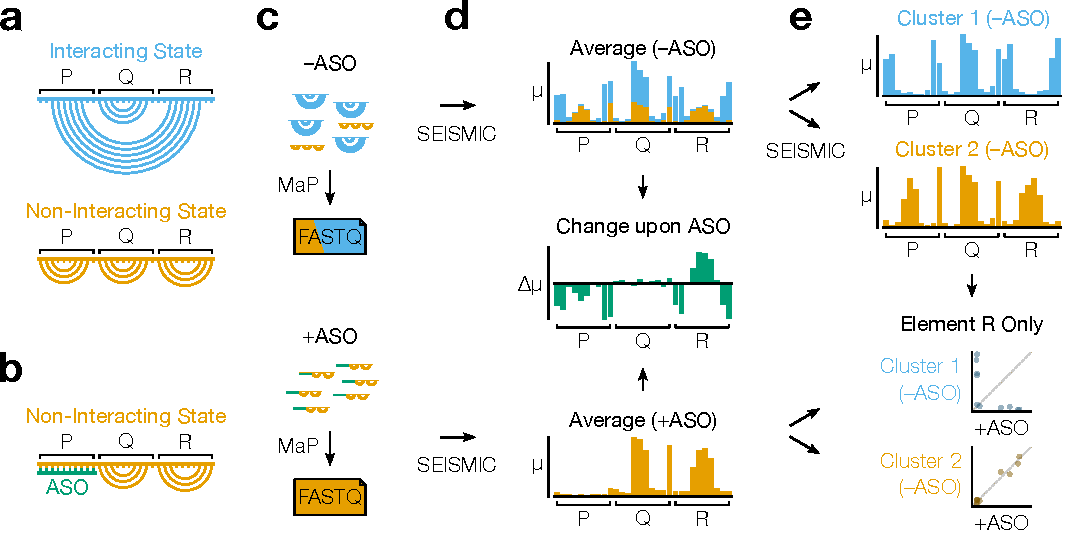
\includegraphics[width=\textwidth]{../MainFigures/strat.pdf}
	\caption{\textbf{The strategy of SEARCH-MaP and SEISMIC-RNA.} \textbf{(a)}~This toy RNA is partitioned into three 10 nt elements (P, Q, and R) whose molecules exist in two structural states: one in which elements P and R interact (blue) and one in which they do not (orange). \textbf{(b)}~Hybridizing an ASO (green) to element P blocks it from interacting with element R and forces all RNA molecules into the non-interacting state. \textbf{(c)} A SEARCH-MaP experiment entails separate chemical probing and mutational profiling (MaP) with (+ASO) and without (--ASO) the ASO, followed by sequencing to generate FASTQ files. The RNA molecules and FASTQ files use the same color scheme as in (a) and are illustrated/colored in proportion to their abundances in the ensemble. \textbf{(d)} Ensemble average mutational profiles with (+ASO) and without (--ASO) the ASO, computed with SEISMIC-RNA. The \textit{x}-axis is the position in the RNA sequence; the \textit{y}-axis is the fraction of mutations ($\mu$) at the position. Each bar in the --ASO profile is drawn in two colors merely to illustrate how much each state contributes to each position; in a real experiment, states cannot be distinguished before clustering. The change upon ASO binding (green) indicates the difference in mutation fraction ($\Delta \mu$) between the +ASO and --ASO conditions. \textbf{(e)} Mutational profiles of two clusters (top) obtained by unmixing the --ASO ensemble in (d) using SEISMIC-RNA, and the scatter plot of the mutation rates in element R (bottom) between the +ASO ensemble average (\textit{x}-axis) and each cluster (\textit{y}-axis).}
	\label{strat}
\end{figure}


We illustrate SEARCH-MaP with an RNA comprising three elements (P, Q, and R) that folds into an ensemble of two structural states: one in which elements P and R interact, another in which they do not (Figure~\ref{strat}a).
Searching for RNA--RNA interactions involving element P begins with hybridizing an antisense oligonucleotide (ASO) to element P, which blocks P--R base pairing and ablates the interacting state (Figure~\ref{strat}b).
The perturbation is then detected by chemically probing with (+ASO) and without (--ASO) the ASO, followed by mutational profiling and sequencing, e.g. using DMS-MaPseq~\cite{Zubradt2016} (Figure~\ref{strat}c).

SEISMIC-RNA can detect RNA--RNA interactions by comparing the mutational profiles of +ASO and --ASO conditions.
Theoretically, each structural state has its own mutational profile~\cite{Sherpa2015}, but the mutational profile of a single state is not directly observable because all states are physically mixed during the experiment (Figure~\ref{strat}c, top).
Instead, the directly observable mutational profile is the "ensemble average" -- the average of the states' (unobserved) mutational profiles, weighted by the states' (unobserved) proportions (Figure~\ref{strat}d, top).
Because the structures -- and therefore mutational profiles -- of element R differ between the interacting and non-interacting states, the ensemble averages over element R also differ between the +ASO and --ASO conditions (Figure~\ref{strat}d, middle).
However, this is not the case for element Q, which has the same secondary structure in both states (Figure~\ref{strat}d, middle).
Therefore, one can deduce that P interacts with R -- but not with Q -- because hybridizing an ASO to P alters the mutational profile of R but not of Q.

After identifying RNA--RNA interactions, SEISMIC-RNA can also determine the mutational profiles of the interacting and non-interacting states -- even if their secondary structures are unknown.
Inferring mutational profiles for the interacting and non-interacting states requires unmixing the --ASO ensemble into two clusters of RNA molecules (Figure~\ref{strat}e, top).
Each cluster has its own mutational profile and corresponds to one structural state, but which cluster corresponds to the interacting (or non-interacting) state is not yet known.
The non-interacting state has a mutational profile similar to that of the +ASO ensemble average, since the ASO forces the RNA into the non-interacting state.
Therefore, over the element (in this case, R) that interacts with the ASO-bound element, the cluster that correlates better with the +ASO ensemble average is the non-interacting state (Figure~\ref{strat}e, bottom).
Using this technique, one can deduce that Cluster 2 corresponds to the non-interacting state, and Cluster 1 to the interacting state.


\end{document}
